\documentclass[12pt]{article}
\usepackage[a4paper, margin=1in]{geometry}
\usepackage{graphicx}
\usepackage{hyperref}
\usepackage{titlesec}
\usepackage{enumitem}
\usepackage{fancyhdr}
\usepackage{float}
\usepackage{xcolor}
\usepackage{array}
\usepackage{longtable}
\usepackage{pgfplots}
\usepackage{amssymb}
\usepackage{subcaption}
\usepackage{subcaption} % for side-by-side images
\pgfplotsset{compat=1.18}
\hypersetup{
    colorlinks=true,
    linkcolor=blue,
    urlcolor=blue
}

\pagestyle{fancy}
\fancyhf{}
\rhead{Health Companion Super App}
\lhead{UX/UI Case Study}
\rfoot{\thepage}

\title{\textbf{UX/UI Case Study}\\
Health Companion Super App}
\author{Abdel-Rahman Khalifa \(40253332\)}
\date{\today}

\begin{document}

\maketitle
\tableofcontents
\newpage

% ==================================================
\section{Introduction}

\subsection{App Overview}

Patients living with chronic health conditions often struggle to consistently manage their medications and medical appointments. This challenge becomes more significant during non-routine days or when individuals experience psychological stress, cognitive overload, or personal distractions. Missed doses and forgotten appointments can negatively affect treatment outcomes and overall health stability.

The Health Companion Super App is designed to provide a simple, reliable, and accessible user experience that supports medication adherence and appointment management. The application reduces cognitive load through structured reminders, clear visual hierarchy, and intuitive navigation.

In addition to medication tracking, the app offers quick access to hospital hotlines and personal healthcare providers, positioning it as a centralized health companion. Special emphasis is placed on accessibility, privacy, and trust, ensuring that users feel confident and secure while managing sensitive medical information.

\subsection{Problem Context}
Existing health applications often focus on isolated features such as reminders or appointment booking, but rarely integrate medication management, communication access, and emergency resources into a single cohesive experience. This fragmentation increases cognitive load and reduces long-term engagement.

\subsection{Project Goals}
\begin{itemize}
    \item Increase the likelyhood of on-time medication adherence
    \item Reduce missed medical appointments
    \item Minimize cognitive load associated with health management
    \item Provide a centralized and trustworthy health management platform
    \item Ensure accessibility for elderly users while maintaining efficiency for young people.
\end{itemize}

% ==================================================
\section{User Research}

\subsection{Research Methodology}

Research combined:
\begin{itemize}
    \item Competitive analysis of leading medication management applications
    \item Review mining of publicly available user feedback
    \item Rapid secondary review of medication adherence literature
\end{itemize}

\subsection{Data Sources Overview}

Rather than conducting a primary survey, this study analyzed publicly available 
user reviews from three established medication management applications: 
Medisafe, MyTherapy, and Dosecast.

The collected reviews represent diverse users managing recurring medications, 
including long-term chronic conditions and short-term prescriptions.

\subsection{Key Findings}

\begin{itemize}
    \item Users frequently experience reminder reliability issues
    \item Complex onboarding and multi-step actions create frustration
    \item Excessive notifications lead to disengagement
    \item Users want simple, fast interaction rather than feature-heavy systems
    \item Limited data export and privacy transparency reduce trust
\end{itemize}

To better understand dominant usability pain points, recurring issues were categorized and frequency-counted across analyzed reviews.
\begin{figure}[h]
\centering
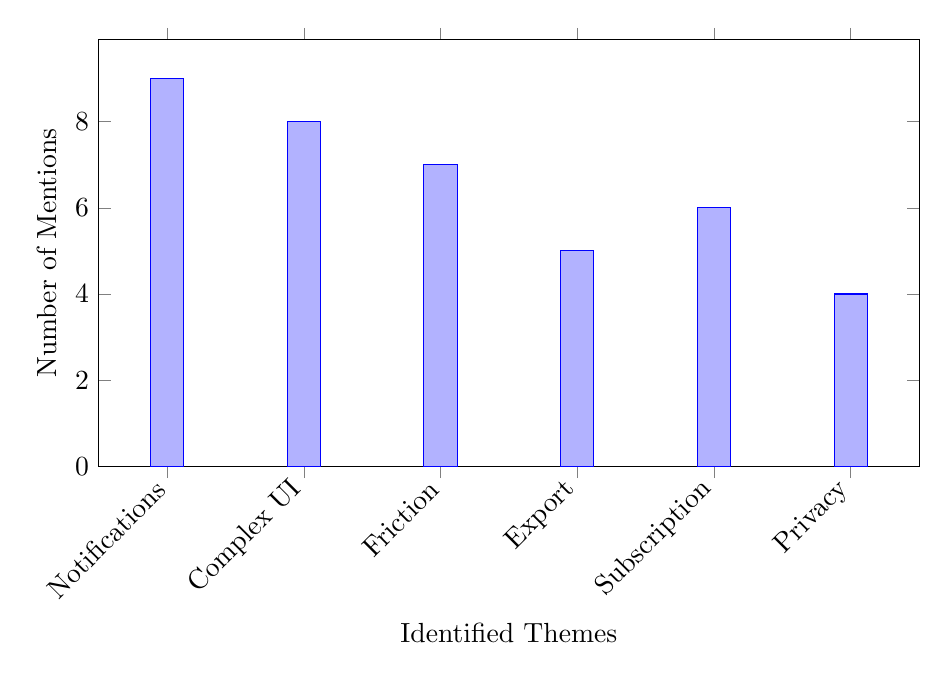
\begin{tikzpicture}
\begin{axis}[
    ybar,
    symbolic x coords={Notifications,Complex UI,Friction,Export,Subscription,Privacy},
    xtick=data,
    ylabel={Number of Mentions},
    xlabel={Identified Themes},
    ymin=0,
    bar width=12pt,
    width=12cm,
    height=7cm,
    xticklabel style={rotate=45, anchor=east}
]
\addplot coordinates {
    (Notifications,9)
    (Complex UI,8)
    (Friction,7)
    (Export,5)
    (Subscription,6)
    (Privacy,4)
};
\end{axis}
\end{tikzpicture}
\caption{Frequency of recurring usability issues identified in cross-application review analysis}
\end{figure}

\subsection{Thematic Analysis}

\begin{longtable}{|p{3cm}|p{4cm}|p{4cm}|}
\hline
\textbf{Theme} & \textbf{Evidence from Review Analysis} & \textbf{Design Impact} \\
\hline
Reminder Reliability & Users report delayed or buggy notifications & High-reliability reminder engine \\
\hline
Interaction Friction & Multi-step confirmations and forced fields frustrate users & One-tap confirmation system \\
\hline
Notification Fatigue & Aggressive or repetitive alerts cause annoyance & Customizable and adaptive alerts \\
\hline
Feature Overload & Interfaces described as cluttered or overwhelming & Minimalist and focused UI design \\
\hline
Data Ownership & Difficulty exporting records and privacy concerns & Simple export and transparent data controls \\
\hline
\end{longtable}


\subsection{Cross-Application Issue Comparison}
\begin{table}[h]
\centering
\caption{Issue presence across analyzed applications}
\begin{tabular}{|l|c|c|c|}
\hline
\textbf{Issue} & \textbf{Medisafe} & \textbf{MyTherapy} & \textbf{Dosecast} \\
\hline
Notification Reliability Issues & \checkmark & \checkmark & \checkmark \\
Complex / Fragmented UI & \checkmark & \checkmark & \checkmark \\
Data Export Limitations & \checkmark & \checkmark & \checkmark \\
Subscription / Premium Friction & \checkmark & \checkmark & \checkmark \\
Forced Login / Cloud Sync & $\times$ & $\times$ & \checkmark \\
Interaction Irreversibility & \checkmark & \checkmark & \checkmark \\
\hline
\end{tabular}
\end{table}

% ==================================================
\section{User Personas}

From the review analysis and competitive research, three main types of users became clear. 
These personas are not fictional characters, but representations of real usage patterns observed in existing medication management apps. 
Each one highlights a different way people interact with these systems: someone who depends on reminders working reliably, someone managing a stable daily routine who wants simplicity, and someone coordinating care for another person.

% ------------------------------
\subsection{Daniel}

Daniel represents users who rely heavily on reminders to manage medication that must be taken at specific times. 
For this group, the biggest concern is reliability. If a reminder fails or is delayed, it is not just inconvenient, it can disrupt their entire day. 
They are less interested in extra features and more concerned with knowing the app will work consistently without needing to double-check it.

\begin{figure}[H]
\centering
\includegraphics[width=0.95\textwidth]{persona1_Daniel.png}
\caption{Persona 1 – Daniel}
\end{figure}

% ------------------------------
\subsection{Linda}

Linda represents users who take medication as part of a long-term, stable routine. 
They use the app mainly as a support tool and prefer something simple that fits naturally into their day. 
Complicated interfaces, extra steps, or frequent design changes can feel frustrating because they interrupt habits that are already established.

\begin{figure}[H]
\centering
\includegraphics[width=0.95\textwidth]{persona2_Linda.png}
\caption{Persona 2 – Linda}
\end{figure}

% ------------------------------
\subsection{Maria}

Maria represents caregivers who are managing medication for someone else, such as a parent or family member. 
In this case, the goal is not just receiving reminders, but being able to see information clearly, coordinate with others, and understand what has already been done. 
These users need shared visibility and clarity rather than personalization or advanced features.

\begin{figure}[H]
\centering
\includegraphics[width=0.95\textwidth]{persona3_Maria.png}
\caption{Persona 3 – Maria}
\end{figure}
% ==================================================
% ==================================================
\section{User Journey Maps}

% ------------------------------
\subsection{Journey Map – Daniel}

\begin{longtable}{|p{3cm}|p{4cm}|p{3cm}|p{4cm}|}
\hline
\textbf{Stage} & \textbf{Action} & \textbf{Emotion} & \textbf{Pain Point} \\
\hline
Realization & Notices reduced focus and realizes he may have missed medication & Concerned, distracted & Cannot immediately confirm whether medication was taken \\
\hline
Verification & Opens the app to check history and sees an earlier reminder & Frustrated & Reminder appeared, but system reliability is unclear \\
\hline
Double-Checking & Re-checks logs multiple times throughout the day to verify doses & Anxious, distracted & Lack of trust forces repeated manual verification \\
\hline
Interruption & Receives a notification but must open the app to confirm it is accurate & Skeptical & Cannot rely on notification alone \\
\hline
Configuration Attempt & Tries to add or adjust medication plan & Overwhelmed & Multi-step forms and unclear workflow \\
\hline
Successful Reminder & Receives a clear, timely notification and logs medication & Relieved but cautious & Needs reassurance the system worked \\
\hline
End of Day & Reflects on time spent checking the app repeatedly & Mentally fatigued & Productivity loss due to low trust in system \\
\hline
\end{longtable}

% ------------------------------
\subsection{Journey Map – Linda}

\begin{longtable}{|p{3cm}|p{4cm}|p{3cm}|p{4cm}|}
\hline
\textbf{Stage} & \textbf{Action} & \textbf{Emotion} & \textbf{Pain Point} \\
\hline
Morning Routine & Opens app as part of daily habit to confirm medication & Calm, habitual & Wants quick confirmation without disruption \\
\hline
Logging Medication & Attempts to mark medication as taken & Mildly annoyed & Too many prompts or confirmation steps \\
\hline
Interface Interaction & Navigates through checkboxes and extra fields & Frustrated & App adds unnecessary complexity to a simple task \\
\hline
Update Encounter & Notices interface changes after an app update & Confused & Familiar workflow has changed unexpectedly \\
\hline
Daily Use & Continues using app but ignores extra features & Resigned & Feature overload does not match needs \\
\hline
Reflection & Feels task should have taken seconds instead of minutes & Impatient & App slows down an already-established routine \\
\hline
\end{longtable}


% ------------------------------
\subsection{Journey Map – Maria}

\begin{longtable}{|p{3cm}|p{4cm}|p{3cm}|p{4cm}|}
\hline
\textbf{Stage} & \textbf{Action} & \textbf{Emotion} & \textbf{Pain Point} \\
\hline
Care Coordination & Checks medication status for her father before visiting & Responsible, focused & Needs quick overview across schedules \\
\hline
Accessing Information & Logs into app from another device & Confused & Account or device restrictions create friction \\
\hline
Verification & Looks for instructions on dosage or timing & Pressured & Information buried in multiple menus \\
\hline
Communication & Attempts to share updates with family members & Frustrated & Limited sharing or export functionality \\
\hline
Monitoring & Reviews whether medication has already been taken & Cautious & No clear shared visibility between caregivers \\
\hline
Daily Management & Uses app as coordination tool rather than reminder system & Task-focused & Designed for individuals, not caregiving workflows \\
\hline
Reflection & Wants a clearer dashboard to avoid mistakes & Concerned & Lack of collaborative design increases cognitive load \\
\hline
\end{longtable}


% ==================================================

% ==================================================
\section{Storyboard}

To provide a clear visualization of the user interaction flow, we developed a storyboard for our persona, Linda, demonstrating how she uses the app to maintain her long-term medication routine and schedule health updates. By leveraging her specific needs for simplicity and stability, this sequence illustrates a design that prioritizes minimal friction and reinforces her established habits. Using a set of strategic prompts that define her preference for a "support tool" over a complex interface, the AI generated this visual narrative of her logical and stress-free daily journey.
\begin{figure}[H]
\centering
\includegraphics[width=0.95\textwidth]{linda_storyboard.png}
\caption{Storyboard – Daily Interaction Flow}
\end{figure}

% ==================================================
\section{User Flow Diagram}

The following diagram represents the navigation and task flow of the application.

\begin{figure}[H]
\centering
\includegraphics[width=0.95\textwidth]{userflow.png}
\caption{User Flow Chart}
\end{figure}

% ==================================================
% ==================================================
\section{Sketches and Wireframes}

\subsection{Low-Fidelity Sketch Iterations}

The design process began with hand-drawn sketches to explore layout ideas and user flow.
Two iterations were created to progressively refine structure, hierarchy, and usability.

\begin{figure}[H]
\centering
\begin{subfigure}[t]{0.45\textwidth}
    \centering
    \includegraphics[width=\textwidth]{sketches1.png}
    \caption{Iteration 1  Initial Concept Exploration}
\end{subfigure}
\hfill
\begin{subfigure}[t]{0.45\textwidth}
    \centering
    \includegraphics[width=\textwidth]{sketches2.png}
    \caption{Iteration 2  Refined Layout and Navigation}
\end{subfigure}
\caption{Evolution of Low-Fidelity Sketches}
\end{figure}

\subsection{Wireframes}

Based on the validated sketches, higher-fidelity wireframes were produced to
translate the conceptual layouts into structured digital designs. These wireframes
focus on defining content placement, navigation flow, and functional grouping
without emphasizing visual styling.

\begin{figure}[H]
\centering

% -------- First Row --------
\begin{subfigure}[t]{0.32\textwidth}
    \centering
    \includegraphics[width=\textwidth]{homewire.png}
    \caption{Home Screen}
\end{subfigure}
\hfill
\begin{subfigure}[t]{0.32\textwidth}
    \centering
    \includegraphics[width=\textwidth]{medswire.png}
    \caption{Medication Reminder}
\end{subfigure}
\hfill
\begin{subfigure}[t]{0.32\textwidth}
    \centering
    \includegraphics[width=\textwidth]{appointmentswire.png}
    \caption{Appointment Scheduling}
\end{subfigure}

\vspace{0.6cm}

% -------- Second Row --------
\begin{subfigure}[t]{0.32\textwidth}
    \centering
    \includegraphics[width=\textwidth]{logswire.png}
    \caption{Medication History}
\end{subfigure}
\hfill
\begin{subfigure}[t]{0.32\textwidth}
    \centering
    \includegraphics[width=\textwidth]{confirmwire.png}
    \caption{Confirmation Screen}
\end{subfigure}
\hfill
\begin{subfigure}[t]{0.32\textwidth}
    \centering
    \includegraphics[width=\textwidth]{caregiverwire.png}
    \caption{Caregiver Interface}
\end{subfigure}

\caption{System Wireframes Overview}
\end{figure}

% ==================================================
\section{UI Design Decisions}

\subsection{Color Palette}

The color system was intentionally limited to a small set of functional colors to reduce cognitive load and maintain clarity for users managing health-related tasks.

\begin{itemize}
\item \textbf{Primary Blue (#2F6FED):} Used for navigation, headers, and key interface elements. Blue was selected because it is commonly associated with trust, stability, and medical environments, reinforcing user confidence in the reliability of reminders and records.

\item \textbf{Confirmation Green (\#24A67B):} Used for successful actions such as marking medication as taken or completing tasks. Green provides a clear, positive feedback signal without being visually overwhelming.

\item \textbf{Neutral Backgrounds (\#F5F7FB, \#FFFFFF):} Light neutral tones create a calm interface and reduce visual fatigue during repeated daily use.

\item \textbf{Support Grays (\#6B7280 and light divider grays):} Used for secondary information, structure, and separation of content, allowing important actions to stand out without excessive contrast.

\end{itemize}

This restrained palette avoids bright or saturated colors that could create stress or distraction, aligning with the goal of a low-friction health companion.

\subsection{Typography}

The interface uses a system sans-serif typeface (iOS system font style such as \textit{SF Pro / Inter / Helvetica Neue equivalents}) to ensure readability, familiarity, and performance across devices.

\begin{itemize}
\item A \textbf{minimum base size of 16px} was selected to support accessibility guidelines and reduce strain for elderly users.

\item \textbf{Clear typographic hierarchy} distinguishes key information:
\begin{itemize}
    \item Larger, bold headings for medication names and primary actions
    \item Medium-weight labels for schedules and appointments
    \item Muted secondary text for contextual information
\end{itemize}

\item Using system fonts ensures faster loading, consistency with native mobile interfaces, and improved usability for users already familiar with smartphone conventions.

\end{itemize}

\subsection{Layout and Interaction Style}

The UI follows a mobile-first, card-based layout inspired by native iOS design patterns.

\begin{itemize}
\item \textbf{Rounded cards and grouped content} visually separate tasks into manageable units, helping users quickly scan information.

\item \textbf{Single-action screens} minimize decision complexity (e.g., one-tap medication confirmation).

\item \textbf{Bottom navigation bar} provides persistent access to core sections (Home, Medications, Appointments, Caregiver, Settings), supporting predictable navigation.

\item \textbf{Generous spacing and padding} reduce accidental taps and support users with limited dexterity.

\end{itemize}

% ==================================================
\section{Prototype}

The interactive prototype was implemented as a lightweight web-based simulation
to validate navigation clarity, task flow, and interaction simplicity before any
full development effort.

\textbf{Live Prototype:} \url{https://abdelrahmanwm.github.io/MiniProjProto/}

The prototype focuses on validating:
\begin{itemize}
\item One-tap medication confirmation workflow
\item Reduced cognitive load through simplified layouts
\item Clear navigation between the five core sections
\item Caregiver visibility and coordination features
\end{itemize}

\begin{figure}[H]
\centering

% -------- First Row --------
\begin{subfigure}[t]{0.32\textwidth}
    \centering
    \includegraphics[width=\textwidth]{home.png}
    \caption{Home Dashboard}
\end{subfigure}
\hfill
\begin{subfigure}[t]{0.32\textwidth}
    \centering
    \includegraphics[width=\textwidth]{appointments.png}
    \caption{Appointments View}
\end{subfigure}
\hfill
\begin{subfigure}[t]{0.32\textwidth}
    \centering
    \includegraphics[width=\textwidth]{meds.png}
    \caption{Medication List}
\end{subfigure}

\vspace{0.6cm}

% -------- Second Row --------
\begin{subfigure}[t]{0.32\textwidth}
    \centering
    \includegraphics[width=\textwidth]{caregiver.png}
    \caption{Caregiver Dashboard}
\end{subfigure}
\hfill
\begin{subfigure}[t]{0.32\textwidth}
    \centering
    \includegraphics[width=\textwidth]{confirm.png}
    \caption{Dose Confirmation}
\end{subfigure}
\hfill
\begin{subfigure}[t]{0.32\textwidth}
    \centering
    \includegraphics[width=\textwidth]{log.png}
    \caption{Medication History}
\end{subfigure}

\caption{Interactive Prototype Screens}
\end{figure}

% ==================================================
\section{Usability Testing}

\subsection{Testing Plan}
Because this project focused on design and prototyping rather than deployment,
a hypothesis-driven evaluation was used instead of formal usability testing.
This approach assesses whether the design decisions logically address the
usability problems identified during research.

\subsection{Evaluation Rationale}

Prior review analysis revealed that existing medication-management applications
suffer from:
\begin{itemize}
    \item Multi-step interaction flows that increase friction
    \item Visual and functional overload
    \item Lack of trust caused by unclear system feedback
\end{itemize}

The prototype was therefore designed to intentionally reduce interaction depth,
limit interface complexity, and emphasize clear confirmation states.

\subsection{Design Hypotheses}

The following hypotheses guided the interface design:

\textbf{H1:} A one-tap medication confirmation flow will reduce cognitive effort
compared to multi-step logging workflows found in competing applications.

\textbf{H2:} A minimal, card-based layout will improve information scanning and
allow users to verify health-related tasks more quickly.

\textbf{H3:} Persistent bottom navigation will provide predictable movement between
tasks, supporting both routine users and caregivers managing another person’s care.

\subsection{Analytical Validation}

The prototype was reviewed against these hypotheses by examining task paths
and interaction cost:

\begin{itemize}
    \item Confirming a medication requires a single action from the home screen,
    eliminating navigation depth.
    \item Each screen presents one primary purpose, avoiding feature competition.
    \item Information is grouped into discrete cards, enabling rapid visual parsing.
    \item Caregiver functionality emphasizes visibility rather than configuration,
    aligning with coordination-focused usage.
\end{itemize}

\subsection{Expected Outcomes}

Based on established usability principles (Hick’s Law, Cognitive Load Theory,
and Recognition-over-Recall interaction models), the design is expected to:

\begin{itemize}
    \item Reduce decision time for recurring tasks
    \item Improve adherence through predictable confirmation feedback
    \item Lower user fatigue during repeated daily interactions
\end{itemize}

This hypothesis-based evaluation provides a reasoned validation of the design
prior to real-world testing, which would be the next phase in a production setting.

% ==================================================
% ==================================================
\section{Reflection}

This project demonstrated how small usability frictions can significantly affect adherence behaviors in health-related contexts. By grounding design decisions in real user feedback rather than feature expansion, the final solution emphasizes reliability, clarity, and low cognitive demand. The iterative process reinforced that, for routine-driven applications, reducing interaction complexity is more valuable than adding functionality.

% ==================================================
% ==================================================
\section{Conclusion}

The Health Companion Super App illustrates a user-centered approach to designing for consistency-driven tasks such as medication adherence and care coordination. Through research synthesis, persona modeling, workflow simplification, and iterative prototyping, the design prioritizes trust, accessibility, and efficiency over feature density. The resulting system provides a focused, scalable foundation for supporting both independent users and caregivers in managing daily health responsibilities.

\end{document}